\documentclass[12pt,fleqn]{article}\usepackage{../common}
\begin{document}
Fourier Transformu ve DFT

Unlu matematikci Fourier sunu kesfetmisti; periyodik olan bir fonksiyon F(x)
sinus ve cosinus terimlerinin toplami olarak temsil edilebilir.

$$ F(x) = a_o + \sum_{n=1}^{\infty}a_n \cos nx + \sum_{n=1}^{\infty}b_n \sin nx  $$

Bu fonksiyonda a ve b sayi degerlerinin bilinmesi gerekmektedir. Onlari nasil
buluruz? 

$a_k$ degerlerini bulmak icin iki tarafi $\cos kx$ ile carpip
$\int_{-\pi}^{\pi}$ ile entegralini alirsak,

$$ \int_{-\pi}^{\pi} F(x)\cos kx \ dx = \int_{-\pi}^{\pi} a_0 \cos
kx \ dx +  \sum_{n=1}^{\infty}\int_{-\pi}^{\pi} a_n \cos nx \cos kx \ dx +   $$

$$ \sum_{n=1}^{\infty}\int_{-\pi}^{\pi} a_n \sin nx \cos kx \ dx   $$

Esitligin sag tarafinda birinci terim $\cos(kx)$, $\sin(kx)$'e donusur. Fakat sinus
fonksiyonu $\pi$ ve $-\pi$ noktalarinda (ya da onlarin k ile carpilmis $2\pi$,
$-2\pi$, vs. gibi katlarinda) sifir degerine sahip oldugu icin, bu terim tamamen
sifir olacaktir, formulden atilabilir.

Ikinci terimde $\cos(nx)\cos(kx)$'in ustteki gibi entegrali eger k ve n esit
degilse, sifirdir. Sadece n ve k esit ise $a_k(\cos kx)^2$ degeri elde edilir.
$(\cos kx)^2$'in iseustteki sekilde entegrali $\pi$ sonucunu verir. Yani ikinci
terimde olan, o sonsuza kadar giden koca toplam icinde sadece tek bir terim sag
kalabilir.

Ucuncu terimde $\sin nx \cos kx$ carpiminin entegrali her zaman
sifir degerini dondurur. Bu terim de formulden atilir. Geri kalanlari tekrar
duzenlersek, 

$$ a_k = \int_{-\pi}^{\pi} F(x)\cos kx \ dx $$

sonucunu elde ederiz. $b_k$ icin benzer islemler, ama bu sefer $\sin kx$ ile carpilarak yapilirsa ve
sonuc asagi yukari ayni.

$$ b_k = \int_{-\pi}^{\pi} F(x)\sin kx \ dx $$

$a_0$ icin ise, $\cos kx$ ya da $\sin kx$ ile carpmaya gerek yok. Sadece iki
tarafin entegralini almak yeterli, $a_o$'i istedigimiz icin $n=0$ demektir, o
zaman sin ve cos iceren hicbir terime ihtiyac yoktur.

$$  \int_{-\pi}^{\pi} F(x) dx =  \int_{-\pi}^{\pi} a_o dx $$
$$  =  a_o x \ \bigg|_{-\pi}^{\pi}  $$
$$  = a_0 (\pi -(-\pi))  $$
$$  = 2\pi a_0  $$

Yani

$$ a_0 = \frac{1}{2\pi}\int_{-\pi}^{\pi}F(x)dx $$

Kompleks Sayilari Kullanmak

$a_o$, $a_n$ ve $b_n$ yerine tek bir $c_n$ turu sayi kullanmak istersek,
kompleks sayi sistemine gecmek lazim. O zaman ilk $F(x)$ formulunu de
donusturmemiz lazim.

Trigonometrik fonksiyonlarda bilinen iki esitlik soyledir:

$$ \cos(\theta) = \frac{e^{i\theta}+e^{-i\theta}}{2} $$

$$ \sin(\theta) = \frac{e^{i\theta}-e^{-i\theta}}{2i}  $$

Bu formulde $i$ degeri hayali sayi olarak bilinen $\sqrt{-1}$ degeridir. 

$F(x)$ formulunu ustteki trigonometrik esitliklere gore donusturelim. 

$$ F(x) = .. +  \sum_{n=1}^{\infty}a_n \cos nx + \sum_{n=1}^{\infty}b_n \sin nx $$

$$ = .. + \sum_{n=1}^{\infty} a_n \frac{e^{inx} + e^{-inx}}{2} +  \sum_{n=1}^{\infty} b_n \frac{e^{inx} - e^{-inx}}{2i}\\ $$

$$ = .. + \sum_{n=1}^{\infty} \frac{a_ne^{inx}}{2} + \frac{a_ne^{-inx}}{2} +
\frac{b_ne^{inx}}{2i} - \frac{b_ne^{-inx}}{2i} $$

$$ = .. + \sum_{n=1}^{\infty} \frac{a_ne^{inx}}{2} + \frac{a_ne^{-inx}}{2} -
\frac{i \ b_ne^{inx}}{2} + \frac{ \ b_ne^{-inx}}{2} $$

Benzer terimleri, yani $e^{inx}$ ve $e^{-inx}$ terimlerini beraber yazalim:

$$ = .. + \sum_{n=1}^{\infty} \frac{a_n-b_ni}{2}e^{inx} + \frac{a_n+b_ni}{2}e^{-inx} $$

Bolumde olan $2i$ icindeki $i$ nasil yukari cikabildi? Bu durum, hayali
sayilarin bir ozelligiyle alakali: $1/i = -i$. Boylece ikinci ve dorduncu
terimdeki arti ve eksi isaretleri degismis oldu. Daha kisa yazmak icin

$$ c_{-n} = \frac{a_n + b_n}{2} $$

$$ c_{n} = \frac{a_n - b_n}{2} $$

olarak temsil edersek

$$F(x) = \sum_{n=-\infty}^{\infty} c_ne^{inx} $$

Ustteki $c_{-n}$ ve $c_n$ kullanimi bize ek bir avantaj sagliyor:
$-inx$ ibaresindeki eksi degeri de cekip cikartabiliyoruz, eksi deger
$i$'den alinip $n$'ye veriliyor yani, ve eksilik toplamdaki alt sinir
olarak tanimlaniyor. Nasil olsa final formulde $i$ ve $n$ carpildigi
icin sonuc degismiyecek, ve tek bir terim kullanabilecegiz. Ek olarak
$a_0$ ise $c_o$ haline geldi.

Ustteki entegralli teknigin benzerini $c_n$ icin de
kullanabiliriz. Esitligin sag tarafindaki kisim ustteki formulde
$\Sigma$ toplaminin acilmis halini kullanalim, ve iki tarafi da
$e^{-ikx}$ ile carpalim, sonra $-\pi$ ve $\pi$ arasinda entegralini
alalim:

$$ \int_{-\pi}^{\pi}F(x)e^{-ikx}dx = \int_{-\pi}^{\pi}c_0e^{-ikx}dx + $$

$$ \int_{-\pi}^{\pi}c_1e^{ix}e^{-ikx}dx + ... +  $$

$$ \int_{-\pi}^{\pi}c_ke^{ikx}e^{-ikx}dx + ... $$

Toplamdaki tum terimleri gostermedik, onemli olan kisim zaten k'inci terim, yani
$e^{-ikx}$ ile carpilan $e^{ikx}$ ifadesi. Bu carpim basit bir cebirsel islemle
$e^{-ikx}e^{ikx} = e^{-ikx + ikx} = e^{0} = 1$, yani bir degerine esit. Diger
tum terimler eger entegrali hesaplarsak gorebilecegimiz gibi sifira esit. Bir
degerinin$-\pi$ ve $\pi$ arasinda entegrali $2\pi$. Geri kalanlar

O zaman

$$ 2\pi c_k = \int_{-\pi}^{\pi}F(x)e^{-ikx}dx $$

$$ c_k = \frac{1}{2\pi}\int_{-\pi}^{\pi}F(x)e^{-ikx}dx $$

Sifira esitligin nasil oldugunu cebirsel olarak gosterelim. Entegrali alalim,

$$ \int_{-\pi}^{\pi}e^{inx}e^{-ikx}dx $$

$$ = \int_{-\pi}^{\pi}e^{i(n-k)x}dx $$

$$ = \frac{e^{i(n-k)x}}{i(n-k)} \bigg|_{-\pi}^{\pi}  $$

$$ = e^{in\pi}e^{-ik\pi} - e^{-in\pi}e^{ik\pi} = 0 $$

DFT

Ayriksal (discrete) olarak Fourier modellemesi yapmak istiyorsak, elimizde
devamli (continuous) f(x) fonksiyonu olmayacak, bir f(x) fonksiyonun belli
noktalarindaki degerleri (oldugunu farzettigimiz) verileri iceren bir 
*vektor* olacak. Bu vektorun N elemani var diyelim. Fonksiyon periyodik
olduguna gore, x icin $2\pi$'i N esit parcaya boleriz (tahtadan alinan resim
altta). Ornegimizde N=4 olsun.

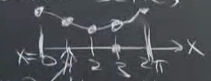
\includegraphics[height=3cm]{four.png}

Ayrica $F(x)$ formulu biraz degisecek. Elimizde sonsuz tane nokta olmadigina gore

$$ F(x) = \sum_{n=0}^{N} c_ne^{inx} $$

olmasi lazim. Simdi, eger butun $c_k$ degerlerini biliyor olsaydik, bu
fonksiyon, x=0 noktasinda hangi degere sahip olurdu?

$$ f(0) = c_0 + c_1 + c_2 + c_3 + c_4 = Y_0 $$

Sonraki x degerleri $2\pi/N$, $4\pi/N$ icin asagidaki gibi devam edecegiz, ama
ondan once bir $w$ degiskeni tanimlayalim, bu degiskeni $w=e^{2\pi i/N}$ olarak
alalim. Boylece $w^2$ dedigimizde ustel islemlerde carpim islemi toplama
islemine donusecegi icin $e^{4i\pi/N}$ degeri elde edilebilir, $w^3$ ile
$e^{6i\pi/N}$ elde edilir, vs. Bu degerler bize lazim olacak degerler, $w$
sayesinde formuller daha temiz olacak. $F(2\pi/N)$ icindeki 3. terim ($n=2$)
nedir?  $c_ne^{inx} = c_2e^{2i2\pi/N} = c_2e^{4i\pi/N} = c_2w^2$. O zaman

$$ f(2\pi/N) = c_o + wc_1 + w^2c_2 + w^3c_3 = Y_1 $$

Devam edelim:

$$ f(4\pi/N) = c_o + w^2c_1 + w^4c_2 + w^6c_3 = Y_2  $$

$$ f(6\pi/N) = c_o + w^3c_1 + w^6c_2 + w^9c_3 = Y_3  $$

Elimizdeki dort toplam islemine bakinca, bu toplamlar ve carpimlarin aslinda
lineer cebir uzerinden matrisler ile gosterilebildigini farkedebiliriz. 

$$  
\left[ \begin{array}{c}
    Y_0 \\
    Y_1 \\
    Y_2 \\
    Y_3
\end{array} \right]
=
\left[ \begin{array}{cccc}
    1 & 1 & 1 & 1 \\
    1 & w & w^2 & w^3  \\
    1 & w^2 & w^4 & w^6  \\
    1 & w^3 & w^6 & w^9  
\end{array} \right]
\left[ \begin{array}{c}
    c_0 \\
    c_1 \\
    c_2 \\
    c_3
\end{array} \right] \\
$$

Her matris icin bir degisken kullanirsak

$$ Y = WC $$

F(x)'ten (yani Y'den) C'ye gitmek istersek, elimizde $Y_n$ degerleri var, $w$
degerleri zaten sabittir, W bu sabit degere gore olusturulur, o zaman, $c_n$
sayilarini nasil buluruz?

$$ Y = WC  $$

$$ W^{-1}Y = W^{-1}WC  $$

$$ W^{-1}Y = C $$

Yani $W$ matrisinin tersini (inverse) alip, onu $Y$ ile carpinca elimize $C$
degerleri gececek. 

Gunes Benekleri

Guneste periyodik olarak olan benekler, asagi yukari 11 senede bir ortaya
cikarlar. Bu benekler uzun suredir gozlenmekte ve olculmektedir,
siddetlerine gore, \verb!sunspots.dat! adli dosyada bulabiliriz. Benek
verisindeki periyodik olus, Fourier transformu ile analiz etmek icin
uygun. Alttaki Python kodu $w$, $W$ gibi kavramlari kullanarak, ustteki
carpimlarla $C$ vektorunu bulacak. Bu vektor icindeki sayilar Fourier
analizindeki belli frekanslara, harmoniklere tekabul ediyor olacaklar.

Bu C degerlerinden bazilari digerlerinden daha guclu bir etkidir, mesela 11
senelik periyot, C icinde daha guclu olarak cikacaktir, cikmalidir. Biz kabaca
ilk ve son 30 sayi haricindekileri silerek onlara sifir degeri verdik, sonra bu
yeni C'yi kullanarak benek verisini tekrar "urettirdik". Sonuc onemli olan
(ilk ve son 30 degerin temsil ettigi harmoniklerin onemli oldugunu varsayiyoruz)
periyotlarin yeni bir toplami oldu. Her iki grafigi de ust uste cizdik ve
cakisma oldugunu net bir sekilde gorebiliyoruz. Eger tum C'leri kullansaydik, o
zaman iki grafik daha benzer, hatta tipatip ayni cikacakti.

\begin{minted}{python}
import scipy

tempdata = np.loadtxt("sunspots.dat")

year=tempdata[:,0]

Y=tempdata[:,1]

N = len(Y)

w = np.exp((2*np.pi*1j)/N)

W = np.zeros((N,N), complex)
for i in range(N):
    for k in range(N):
        W[i,k] = w**(i*k)
        
C = np.dot(np.linalg.inv(W), Y) 

C[30:-30] = 0.

Y_new = scipy.real(np.dot(W, C))

plt.plot(year, Y, 'g')
plt.hold(True)
plt.plot(year, Y_new, 'r')
plt.savefig('fourier_1.png')
\end{minted}

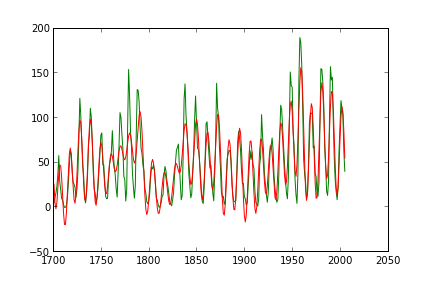
\includegraphics[height=6cm]{fourier_1.png}

FFT

Bitirmeden once FFT konusundan bahsedelim. $\textbf{D}$FT algoritmasi
kodda goruldugu gibi bir W matrisi ortaya cikarir ve once tersini
alma, sonra bu ters ile bir carpim islemi yaparak C sonucunu
uretir. $O$ notasyonunu kullanirsak DFT'nin karmasikligi
$O(N^2)$'dir. Bu iyi bir hizdir.

FFT algoritmasi ustteki carpimin bazi ozelliklerini kullanarak DFT'yi
daha da hizlandirir ve $O(\frac{1}{2}Nlog_2N)$ hizina getirir. FFT'den
bu makalede bahsetmeyecegiz, aklimizda olsun, Scipy uzerinde fft
cagrisi bu algoritmayi kullanir.

Kaynaklar

Strang, G., OCW MIT Lecture \#30, Computational Science and Engineering

Strang, G., Computational Science and Engineering, sf. 340-370

Chu, E., Discrete and Continuous Fourier Transforms

Kammler, D., A First Course in Fourier Analysis

Mattuck, A., OCW MIT Lecture \#17-19, Differential Equations


\end{document}


